\documentclass[1p]{elsarticle_modified}
%\bibliographystyle{elsarticle-num}

%\usepackage[colorlinks]{hyperref}
%\usepackage{abbrmath_seonhwa} %\Abb, \Ascr, \Acal ,\Abf, \Afrak
\usepackage{amsfonts}
\usepackage{amssymb}
\usepackage{amsmath}
\usepackage{amsthm}
\usepackage{scalefnt}
\usepackage{amsbsy}
\usepackage{kotex}
\usepackage{caption}
\usepackage{subfig}
\usepackage{color}
\usepackage{graphicx}
\usepackage{xcolor} %% white, black, red, green, blue, cyan, magenta, yellow
\usepackage{float}
\usepackage{setspace}
\usepackage{hyperref}

\usepackage{tikz}
\usetikzlibrary{arrows}

\usepackage{multirow}
\usepackage{array} % fixed length table
\usepackage{hhline}

%%%%%%%%%%%%%%%%%%%%%
\makeatletter
\renewcommand*\env@matrix[1][\arraystretch]{%
	\edef\arraystretch{#1}%
	\hskip -\arraycolsep
	\let\@ifnextchar\new@ifnextchar
	\array{*\c@MaxMatrixCols c}}
\makeatother %https://tex.stackexchange.com/questions/14071/how-can-i-increase-the-line-spacing-in-a-matrix
%%%%%%%%%%%%%%%

\usepackage[normalem]{ulem}

\newcommand{\msout}[1]{\ifmmode\text{\sout{\ensuremath{#1}}}\else\sout{#1}\fi}
%SOURCE: \msout is \stkout macro in https://tex.stackexchange.com/questions/20609/strikeout-in-math-mode

\newcommand{\cancel}[1]{
	\ifmmode
	{\color{red}\msout{#1}}
	\else
	{\color{red}\sout{#1}}
	\fi
}

\newcommand{\add}[1]{
	{\color{blue}\uwave{#1}}
}

\newcommand{\replace}[2]{
	\ifmmode
	{\color{red}\msout{#1}}{\color{blue}\uwave{#2}}
	\else
	{\color{red}\sout{#1}}{\color{blue}\uwave{#2}}
	\fi
}

\newcommand{\Sol}{\mathcal{S}} %segment
\newcommand{\D}{D} %diagram
\newcommand{\A}{\mathcal{A}} %arc


%%%%%%%%%%%%%%%%%%%%%%%%%%%%%5 test

\def\sl{\operatorname{\textup{SL}}(2,\Cbb)}
\def\psl{\operatorname{\textup{PSL}}(2,\Cbb)}
\def\quan{\mkern 1mu \triangleright \mkern 1mu}

\theoremstyle{definition}
\newtheorem{thm}{Theorem}[section]
\newtheorem{prop}[thm]{Proposition}
\newtheorem{lem}[thm]{Lemma}
\newtheorem{ques}[thm]{Question}
\newtheorem{cor}[thm]{Corollary}
\newtheorem{defn}[thm]{Definition}
\newtheorem{exam}[thm]{Example}
\newtheorem{rmk}[thm]{Remark}
\newtheorem{alg}[thm]{Algorithm}

\newcommand{\I}{\sqrt{-1}}
\begin{document}

%\begin{frontmatter}
%
%\title{Boundary parabolic representations of knots up to 8 crossings}
%
%%% Group authors per affiliation:
%\author{Yunhi Cho} 
%\address{Department of Mathematics, University of Seoul, Seoul, Korea}
%\ead{yhcho@uos.ac.kr}
%
%
%\author{Seonhwa Kim} %\fnref{s_kim}}
%\address{Center for Geometry and Physics, Institute for Basic Science, Pohang, 37673, Korea}
%\ead{ryeona17@ibs.re.kr}
%
%\author{Hyuk Kim}
%\address{Department of Mathematical Sciences, Seoul National University, Seoul 08826, Korea}
%\ead{hyukkim@snu.ac.kr}
%
%\author{Seokbeom Yoon}
%\address{Department of Mathematical Sciences, Seoul National University, Seoul, 08826,  Korea}
%\ead{sbyoon15@snu.ac.kr}
%
%\begin{abstract}
%We find all boundary parabolic representation of knots up to 8 crossings.
%
%\end{abstract}
%\begin{keyword}
%    \MSC[2010] 57M25 
%\end{keyword}
%
%\end{frontmatter}

%\linenumbers
%\tableofcontents
%
\newcommand\colored[1]{\textcolor{white}{\rule[-0.35ex]{0.8em}{1.4ex}}\kern-0.8em\color{red} #1}%
%\newcommand\colored[1]{\textcolor{white}{ #1}\kern-2.17ex	\textcolor{white}{ #1}\kern-1.81ex	\textcolor{white}{ #1}\kern-2.15ex\color{red}#1	}

{\Large $\underline{12n_{0804}~(K12n_{0804})}$}

\setlength{\tabcolsep}{10pt}
\renewcommand{\arraystretch}{1.6}
\vspace{1cm}\begin{tabular}{m{100pt}>{\centering\arraybackslash}m{274pt}}
\multirow{5}{120pt}{
	\centering
	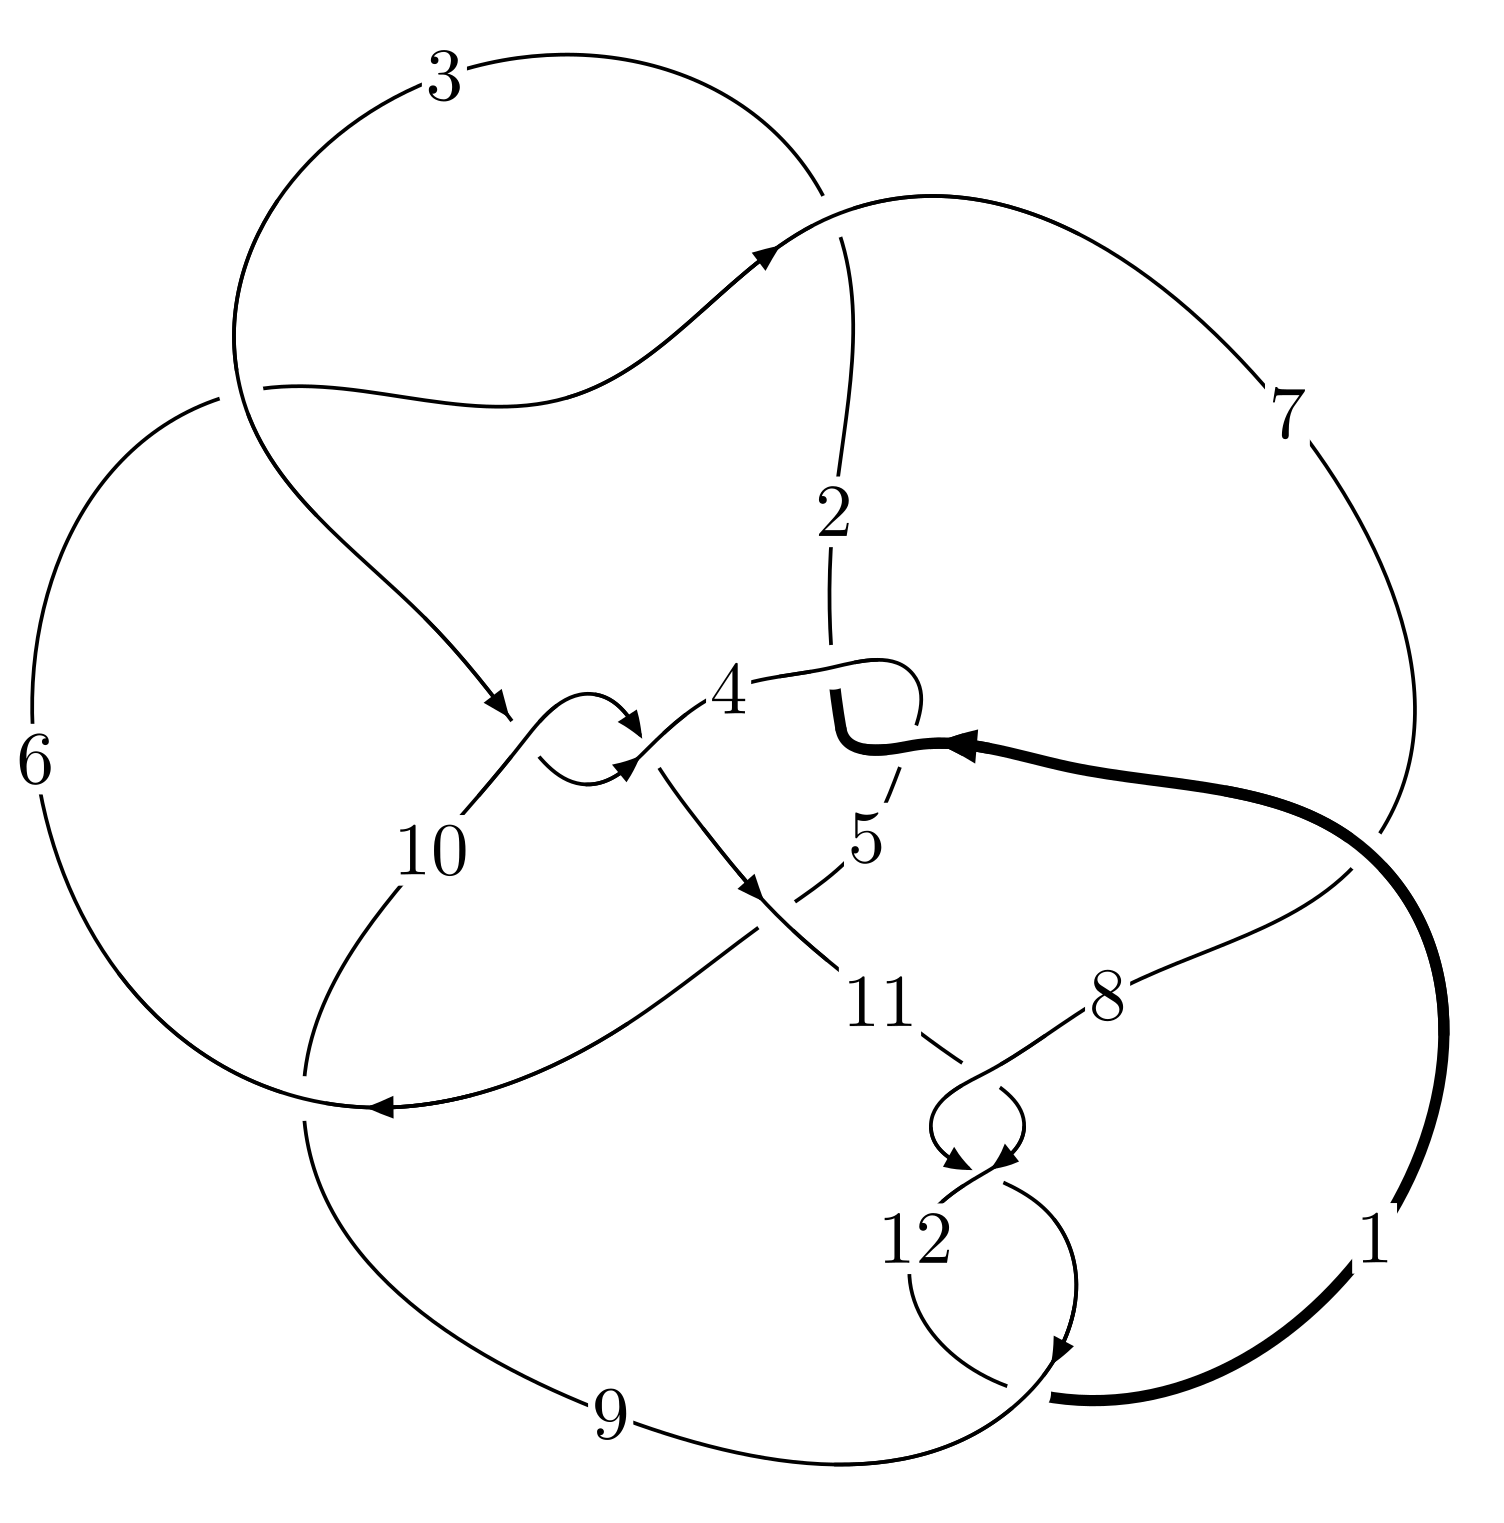
\includegraphics[width=112pt]{../../../GIT/diagram.site/Diagrams/png/2893_12n_0804.png}\\
\ \ \ A knot diagram\footnotemark}&
\allowdisplaybreaks
\textbf{Linearized knot diagam} \\
\cline{2-2}
 &
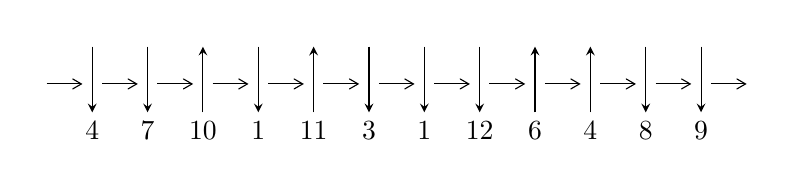
\begin{tikzpicture}[x=20pt, y=17pt]
	% nodes
	\node (C0) at (0, 0) {};
	\node (C1) at (1, 0) {};
	\node (C1U) at (1, +1) {};
	\node (C1D) at (1, -1) {4};

	\node (C2) at (2, 0) {};
	\node (C2U) at (2, +1) {};
	\node (C2D) at (2, -1) {7};

	\node (C3) at (3, 0) {};
	\node (C3U) at (3, +1) {};
	\node (C3D) at (3, -1) {10};

	\node (C4) at (4, 0) {};
	\node (C4U) at (4, +1) {};
	\node (C4D) at (4, -1) {1};

	\node (C5) at (5, 0) {};
	\node (C5U) at (5, +1) {};
	\node (C5D) at (5, -1) {11};

	\node (C6) at (6, 0) {};
	\node (C6U) at (6, +1) {};
	\node (C6D) at (6, -1) {3};

	\node (C7) at (7, 0) {};
	\node (C7U) at (7, +1) {};
	\node (C7D) at (7, -1) {1};

	\node (C8) at (8, 0) {};
	\node (C8U) at (8, +1) {};
	\node (C8D) at (8, -1) {12};

	\node (C9) at (9, 0) {};
	\node (C9U) at (9, +1) {};
	\node (C9D) at (9, -1) {6};

	\node (C10) at (10, 0) {};
	\node (C10U) at (10, +1) {};
	\node (C10D) at (10, -1) {4};

	\node (C11) at (11, 0) {};
	\node (C11U) at (11, +1) {};
	\node (C11D) at (11, -1) {8};

	\node (C12) at (12, 0) {};
	\node (C12U) at (12, +1) {};
	\node (C12D) at (12, -1) {9};
	\node (C13) at (13, 0) {};

	% arrows
	\draw[->,>={angle 60}]
	(C0) edge (C1) (C1) edge (C2) (C2) edge (C3) (C3) edge (C4) (C4) edge (C5) (C5) edge (C6) (C6) edge (C7) (C7) edge (C8) (C8) edge (C9) (C9) edge (C10) (C10) edge (C11) (C11) edge (C12) (C12) edge (C13) ;	\draw[->,>=stealth]
	(C1U) edge (C1D) (C2U) edge (C2D) (C3D) edge (C3U) (C4U) edge (C4D) (C5D) edge (C5U) (C6U) edge (C6D) (C7U) edge (C7D) (C8U) edge (C8D) (C9D) edge (C9U) (C10D) edge (C10U) (C11U) edge (C11D) (C12U) edge (C12D) ;
	\end{tikzpicture} \\
\hhline{~~} \\& 
\textbf{Solving Sequence} \\ \cline{2-2} 
 &
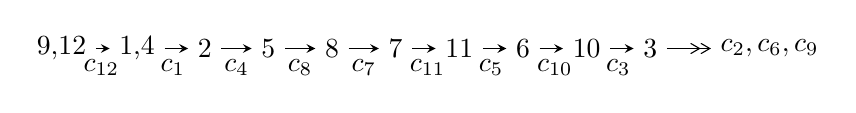
\begin{tikzpicture}[x=23pt, y=7pt]
	% node
	\node (A0) at (-1/8, 0) {9,12};
	\node (A1) at (17/16, 0) {1,4};
	\node (A2) at (17/8, 0) {2};
	\node (A3) at (25/8, 0) {5};
	\node (A4) at (33/8, 0) {8};
	\node (A5) at (41/8, 0) {7};
	\node (A6) at (49/8, 0) {11};
	\node (A7) at (57/8, 0) {6};
	\node (A8) at (65/8, 0) {10};
	\node (A9) at (73/8, 0) {3};
	\node (C1) at (1/2, -1) {$c_{12}$};
	\node (C2) at (13/8, -1) {$c_{1}$};
	\node (C3) at (21/8, -1) {$c_{4}$};
	\node (C4) at (29/8, -1) {$c_{8}$};
	\node (C5) at (37/8, -1) {$c_{7}$};
	\node (C6) at (45/8, -1) {$c_{11}$};
	\node (C7) at (53/8, -1) {$c_{5}$};
	\node (C8) at (61/8, -1) {$c_{10}$};
	\node (C9) at (69/8, -1) {$c_{3}$};
	\node (A10) at (11, 0) {$c_{2},c_{6},c_{9}$};

	% edge
	\draw[->,>=stealth]	
	(A0) edge (A1) (A1) edge (A2) (A2) edge (A3) (A3) edge (A4) (A4) edge (A5) (A5) edge (A6) (A6) edge (A7) (A7) edge (A8) (A8) edge (A9) ;
	\draw[->>,>={angle 60}]	
	(A9) edge (A10);
\end{tikzpicture} \\ 

\end{tabular} \\

\footnotetext{
The image of knot diagram is generated by the software ``\textbf{Draw programme}" developed by Andrew Bartholomew(\url{http://www.layer8.co.uk/maths/draw/index.htm\#Running-draw}), where we modified some parts for our purpose(\url{https://github.com/CATsTAILs/LinksPainter}).
}\phantom \\ \newline 
\centering \textbf{Ideals for irreducible components\footnotemark of $X_{\text{par}}$} 
 
\begin{align*}
I^u_{1}&=\langle 
-15 u^{27}-74 u^{26}+\cdots+2 b+46,\;7 u^{27}+28 u^{26}+\cdots+4 a-16,\;u^{28}+6 u^{27}+\cdots-2 u-4\rangle \\
I^u_{2}&=\langle 
-26336 u^8 a^3-36861 u^8 a^2+\cdots-5783 a+173926,\;-4 u^8 a^2-11 u^8 a+\cdots-3 a+11,\\
\phantom{I^u_{2}}&\phantom{= \langle  }u^9- u^8-4 u^7+3 u^6+5 u^5- u^4-2 u^3-2 u^2+u-1\rangle \\
I^u_{3}&=\langle 
u^{15}- u^{14}-7 u^{13}+5 u^{12}+20 u^{11}-7 u^{10}-27 u^9-4 u^8+12 u^7+15 u^6+8 u^5-3 u^4-7 u^3-8 u^2+b- u,\\
\phantom{I^u_{3}}&\phantom{= \langle  }- u^{16}+u^{15}+\cdots+a-1,\;u^{17}- u^{16}+\cdots- u+1\rangle \\
\\
\end{align*}
\raggedright * 3 irreducible components of $\dim_{\mathbb{C}}=0$, with total 81 representations.\\
\footnotetext{All coefficients of polynomials are rational numbers. But the coefficients are sometimes approximated in decimal forms when there is not enough margin.}
\newpage
\renewcommand{\arraystretch}{1}
\centering \section*{I. $I^u_{1}= \langle -15 u^{27}-74 u^{26}+\cdots+2 b+46,\;7 u^{27}+28 u^{26}+\cdots+4 a-16,\;u^{28}+6 u^{27}+\cdots-2 u-4 \rangle$}
\flushleft \textbf{(i) Arc colorings}\\
\begin{tabular}{m{7pt} m{180pt} m{7pt} m{180pt} }
\flushright $a_{9}=$&$\begin{pmatrix}0\\u\end{pmatrix}$ \\
\flushright $a_{12}=$&$\begin{pmatrix}1\\0\end{pmatrix}$ \\
\flushright $a_{1}=$&$\begin{pmatrix}1\\u^2\end{pmatrix}$ \\
\flushright $a_{4}=$&$\begin{pmatrix}-\frac{7}{4} u^{27}-7 u^{26}+\cdots-\frac{5}{4} u+4\\\frac{15}{2} u^{27}+37 u^{26}+\cdots+\frac{11}{2} u-23\end{pmatrix}$ \\
\flushright $a_{2}=$&$\begin{pmatrix}-6 u^{27}-\frac{61}{2} u^{26}+\cdots-6 u+\frac{45}{2}\\-\frac{27}{2} u^{27}-66 u^{26}+\cdots-\frac{25}{2} u+46\end{pmatrix}$ \\
\flushright $a_{5}=$&$\begin{pmatrix}-\frac{65}{4} u^{27}-72 u^{26}+\cdots-\frac{27}{4} u+41\\-\frac{51}{2} u^{27}-113 u^{26}+\cdots-\frac{17}{2} u+65\end{pmatrix}$ \\
\flushright $a_{8}=$&$\begin{pmatrix}u\\u\end{pmatrix}$ \\
\flushright $a_{7}=$&$\begin{pmatrix}- u^3+2 u\\- u^5+u^3+u\end{pmatrix}$ \\
\flushright $a_{11}=$&$\begin{pmatrix}- u^2+1\\- u^2\end{pmatrix}$ \\
\flushright $a_{6}=$&$\begin{pmatrix}-\frac{23}{4} u^{27}-29 u^{26}+\cdots-\frac{29}{4} u+20\\-\frac{23}{2} u^{27}-56 u^{26}+\cdots-\frac{17}{2} u+37\end{pmatrix}$ \\
\flushright $a_{10}=$&$\begin{pmatrix}2 u^{27}+\frac{17}{2} u^{26}+\cdots- u^2-\frac{7}{2}\\\frac{7}{2} u^{27}+14 u^{26}+\cdots-\frac{1}{2} u-6\end{pmatrix}$ \\
\flushright $a_{3}=$&$\begin{pmatrix}-2 u^{27}-\frac{19}{2} u^{26}+\cdots-2 u+\frac{13}{2}\\\frac{13}{2} u^{27}+31 u^{26}+\cdots+\frac{13}{2} u-20\end{pmatrix}$\\&\end{tabular}
\flushleft \textbf{(ii) Obstruction class $= -1$}\\~\\
\flushleft \textbf{(iii) Cusp Shapes $= -25 u^{27}-119 u^{26}+24 u^{25}+825 u^{24}+445 u^{23}-2632 u^{22}-1414 u^{21}+5532 u^{20}+700 u^{19}-8560 u^{18}+4311 u^{17}+8407 u^{16}-10994 u^{15}-1234 u^{14}+11725 u^{13}-8592 u^{12}-3652 u^{11}+9729 u^{10}-5400 u^9-2649 u^8+5362 u^7-2247 u^6-727 u^5+1376 u^4-434 u^3+57 u^2-28 u+74$}\\~\\
\newpage\renewcommand{\arraystretch}{1}
\flushleft \textbf{(iv) u-Polynomials at the component}\newline \\
\begin{tabular}{m{50pt}|m{274pt}}
Crossings & \hspace{64pt}u-Polynomials at each crossing \\
\hline $$\begin{aligned}c_{1},c_{4}\end{aligned}$$&$\begin{aligned}
&u^{28}-2 u^{27}+\cdots+13 u-1
\end{aligned}$\\
\hline $$\begin{aligned}c_{2},c_{6}\end{aligned}$$&$\begin{aligned}
&u^{28}+20 u^{27}+\cdots-5888 u-512
\end{aligned}$\\
\hline $$\begin{aligned}c_{3},c_{9},c_{10}\end{aligned}$$&$\begin{aligned}
&u^{28}- u^{27}+\cdots+u+1
\end{aligned}$\\
\hline $$\begin{aligned}c_{5}\end{aligned}$$&$\begin{aligned}
&u^{28}+16 u^{26}+\cdots-4 u-11
\end{aligned}$\\
\hline $$\begin{aligned}c_{7}\end{aligned}$$&$\begin{aligned}
&u^{28}-18 u^{27}+\cdots-990 u+52
\end{aligned}$\\
\hline $$\begin{aligned}c_{8},c_{11},c_{12}\end{aligned}$$&$\begin{aligned}
&u^{28}+6 u^{27}+\cdots-2 u-4
\end{aligned}$\\
\hline
\end{tabular}\\~\\
\newpage\renewcommand{\arraystretch}{1}
\flushleft \textbf{(v) Riley Polynomials at the component}\newline \\
\begin{tabular}{m{50pt}|m{274pt}}
Crossings & \hspace{64pt}Riley Polynomials at each crossing \\
\hline $$\begin{aligned}c_{1},c_{4}\end{aligned}$$&$\begin{aligned}
&y^{28}-38 y^{27}+\cdots-43 y+1
\end{aligned}$\\
\hline $$\begin{aligned}c_{2},c_{6}\end{aligned}$$&$\begin{aligned}
&y^{28}+10 y^{27}+\cdots-65536 y+262144
\end{aligned}$\\
\hline $$\begin{aligned}c_{3},c_{9},c_{10}\end{aligned}$$&$\begin{aligned}
&y^{28}-15 y^{27}+\cdots-7 y+1
\end{aligned}$\\
\hline $$\begin{aligned}c_{5}\end{aligned}$$&$\begin{aligned}
&y^{28}+32 y^{27}+\cdots+2096 y+121
\end{aligned}$\\
\hline $$\begin{aligned}c_{7}\end{aligned}$$&$\begin{aligned}
&y^{28}-2 y^{27}+\cdots-384700 y+2704
\end{aligned}$\\
\hline $$\begin{aligned}c_{8},c_{11},c_{12}\end{aligned}$$&$\begin{aligned}
&y^{28}-26 y^{27}+\cdots+4 y+16
\end{aligned}$\\
\hline
\end{tabular}\\~\\
\newpage\flushleft \textbf{(vi) Complex Volumes and Cusp Shapes}
$$\begin{array}{c|c|c}  
\text{Solutions to }I^u_{1}& \I (\text{vol} + \sqrt{-1}CS) & \text{Cusp shape}\\
 \hline 
\begin{aligned}
u &= \phantom{-}0.953650\phantom{ +0.000000I} \\
a &= \phantom{-}0.557977\phantom{ +0.000000I} \\
b &= \phantom{-}1.71191\phantom{ +0.000000I}\end{aligned}
 & -2.95076\phantom{ +0.000000I} & \phantom{-}1.04180\phantom{ +0.000000I} \\ \hline\begin{aligned}
u &= \phantom{-}0.658308 + 0.612846 I \\
a &= -1.282020 - 0.481173 I \\
b &= -1.120110 - 0.609967 I\end{aligned}
 & \phantom{-}0.15275 + 6.58351 I & -2.72995 - 3.03083 I \\ \hline\begin{aligned}
u &= \phantom{-}0.658308 - 0.612846 I \\
a &= -1.282020 + 0.481173 I \\
b &= -1.120110 + 0.609967 I\end{aligned}
 & \phantom{-}0.15275 - 6.58351 I & -2.72995 + 3.03083 I \\ \hline\begin{aligned}
u &= \phantom{-}0.402654 + 0.774191 I \\
a &= -1.05898 - 1.82975 I \\
b &= \phantom{-}0.061414 - 0.574417 I\end{aligned}
 & \phantom{-}1.01000 - 11.30550 I & -1.14807 + 7.82851 I \\ \hline\begin{aligned}
u &= \phantom{-}0.402654 - 0.774191 I \\
a &= -1.05898 + 1.82975 I \\
b &= \phantom{-}0.061414 + 0.574417 I\end{aligned}
 & \phantom{-}1.01000 + 11.30550 I & -1.14807 - 7.82851 I \\ \hline\begin{aligned}
u &= \phantom{-}0.046469 + 0.849926 I \\
a &= -0.926104 - 0.236908 I \\
b &= \phantom{-}0.122562 + 0.203546 I\end{aligned}
 & \phantom{-}6.61374 + 1.82301 I & -2.15341 - 3.95044 I \\ \hline\begin{aligned}
u &= \phantom{-}0.046469 - 0.849926 I \\
a &= -0.926104 + 0.236908 I \\
b &= \phantom{-}0.122562 - 0.203546 I\end{aligned}
 & \phantom{-}6.61374 - 1.82301 I & -2.15341 + 3.95044 I \\ \hline\begin{aligned}
u &= -1.19440\phantom{ +0.000000I} \\
a &= \phantom{-}0.501244\phantom{ +0.000000I} \\
b &= \phantom{-}0.563490\phantom{ +0.000000I}\end{aligned}
 & -2.49793\phantom{ +0.000000I} & -0.727600\phantom{ +0.000000I} \\ \hline\begin{aligned}
u &= \phantom{-}0.323728 + 0.735663 I \\
a &= \phantom{-}1.50512 + 1.36499 I \\
b &= \phantom{-}0.190601 + 0.251246 I\end{aligned}
 & -1.82680 - 3.57508 I & -0.50281 + 5.56081 I \\ \hline\begin{aligned}
u &= \phantom{-}0.323728 - 0.735663 I \\
a &= \phantom{-}1.50512 - 1.36499 I \\
b &= \phantom{-}0.190601 - 0.251246 I\end{aligned}
 & -1.82680 + 3.57508 I & -0.50281 - 5.56081 I\\
 \hline 
 \end{array}$$\newpage$$\begin{array}{c|c|c}  
\text{Solutions to }I^u_{1}& \I (\text{vol} + \sqrt{-1}CS) & \text{Cusp shape}\\
 \hline 
\begin{aligned}
u &= \phantom{-}1.199900 + 0.405002 I \\
a &= -0.456093 - 0.265236 I \\
b &= -1.03504 - 0.98880 I\end{aligned}
 & \phantom{-}3.05496 - 6.32046 I & -4.20827 + 7.87588 I \\ \hline\begin{aligned}
u &= \phantom{-}1.199900 - 0.405002 I \\
a &= -0.456093 + 0.265236 I \\
b &= -1.03504 + 0.98880 I\end{aligned}
 & \phantom{-}3.05496 + 6.32046 I & -4.20827 - 7.87588 I \\ \hline\begin{aligned}
u &= \phantom{-}0.559106 + 0.438994 I \\
a &= \phantom{-}0.554411 + 1.068500 I \\
b &= \phantom{-}0.939165 + 0.581582 I\end{aligned}
 & -2.96704 - 0.44419 I & -3.65164 - 1.30956 I \\ \hline\begin{aligned}
u &= \phantom{-}0.559106 - 0.438994 I \\
a &= \phantom{-}0.554411 - 1.068500 I \\
b &= \phantom{-}0.939165 - 0.581582 I\end{aligned}
 & -2.96704 + 0.44419 I & -3.65164 + 1.30956 I \\ \hline\begin{aligned}
u &= -1.291540 + 0.383259 I \\
a &= -0.271704 + 0.642178 I \\
b &= -0.236794 + 1.202110 I\end{aligned}
 & \phantom{-}2.45039 + 2.60036 I & -6.92230 - 0.38709 I \\ \hline\begin{aligned}
u &= -1.291540 - 0.383259 I \\
a &= -0.271704 - 0.642178 I \\
b &= -0.236794 - 1.202110 I\end{aligned}
 & \phantom{-}2.45039 - 2.60036 I & -6.92230 + 0.38709 I \\ \hline\begin{aligned}
u &= \phantom{-}1.393630 + 0.056371 I \\
a &= \phantom{-}0.117598 + 0.610861 I \\
b &= \phantom{-}0.32341 + 2.06894 I\end{aligned}
 & -5.35082 - 2.09473 I & -9.32900 + 3.91976 I \\ \hline\begin{aligned}
u &= \phantom{-}1.393630 - 0.056371 I \\
a &= \phantom{-}0.117598 - 0.610861 I \\
b &= \phantom{-}0.32341 - 2.06894 I\end{aligned}
 & -5.35082 + 2.09473 I & -9.32900 - 3.91976 I \\ \hline\begin{aligned}
u &= -1.44514 + 0.28991 I \\
a &= -0.09541 - 1.48867 I \\
b &= \phantom{-}0.20048 - 3.17159 I\end{aligned}
 & -7.50725 + 7.32315 I & -4.57096 - 5.41383 I \\ \hline\begin{aligned}
u &= -1.44514 - 0.28991 I \\
a &= -0.09541 + 1.48867 I \\
b &= \phantom{-}0.20048 + 3.17159 I\end{aligned}
 & -7.50725 - 7.32315 I & -4.57096 + 5.41383 I\\
 \hline 
 \end{array}$$\newpage$$\begin{array}{c|c|c}  
\text{Solutions to }I^u_{1}& \I (\text{vol} + \sqrt{-1}CS) & \text{Cusp shape}\\
 \hline 
\begin{aligned}
u &= -1.47470 + 0.16414 I \\
a &= -0.609161 - 0.895856 I \\
b &= -0.02962 - 2.05701 I\end{aligned}
 & -9.43653 + 2.71269 I & -7.85713 + 0. I\phantom{ +0.000000I} \\ \hline\begin{aligned}
u &= -1.47470 - 0.16414 I \\
a &= -0.609161 + 0.895856 I \\
b &= -0.02962 + 2.05701 I\end{aligned}
 & -9.43653 - 2.71269 I & -7.85713 + 0. I\phantom{ +0.000000I} \\ \hline\begin{aligned}
u &= -1.47870 + 0.29110 I \\
a &= \phantom{-}0.46176 + 1.47662 I \\
b &= \phantom{-}0.52784 + 3.55403 I\end{aligned}
 & -5.0564 + 15.1855 I & -4.66281 - 7.85224 I \\ \hline\begin{aligned}
u &= -1.47870 - 0.29110 I \\
a &= \phantom{-}0.46176 - 1.47662 I \\
b &= \phantom{-}0.52784 - 3.55403 I\end{aligned}
 & -5.0564 - 15.1855 I & -4.66281 + 7.85224 I \\ \hline\begin{aligned}
u &= -1.52541 + 0.15808 I \\
a &= \phantom{-}0.112693 + 0.750612 I \\
b &= -0.99764 + 1.57771 I\end{aligned}
 & -7.05591 - 3.93502 I & -6.54817 + 3.13330 I \\ \hline\begin{aligned}
u &= -1.52541 - 0.15808 I \\
a &= \phantom{-}0.112693 - 0.750612 I \\
b &= -0.99764 - 1.57771 I\end{aligned}
 & -7.05591 + 3.93502 I & -6.54817 - 3.13330 I \\ \hline\begin{aligned}
u &= -0.247934 + 0.324230 I \\
a &= \phantom{-}0.668275 - 0.831350 I \\
b &= -0.083982 - 0.333429 I\end{aligned}
 & -0.143060 + 0.866290 I & -3.37260 - 7.97095 I \\ \hline\begin{aligned}
u &= -0.247934 - 0.324230 I \\
a &= \phantom{-}0.668275 + 0.831350 I \\
b &= -0.083982 + 0.333429 I\end{aligned}
 & -0.143060 - 0.866290 I & -3.37260 + 7.97095 I\\
 \hline 
 \end{array}$$\newpage\newpage\renewcommand{\arraystretch}{1}
\centering \section*{II. $I^u_{2}= \langle -2.63\times10^{4} a^{3} u^{8}-3.69\times10^{4} a^{2} u^{8}+\cdots-5783 a+1.74\times10^{5},\;-4 u^8 a^2-11 u^8 a+\cdots-3 a+11,\;u^9- u^8+\cdots+u-1 \rangle$}
\flushleft \textbf{(i) Arc colorings}\\
\begin{tabular}{m{7pt} m{180pt} m{7pt} m{180pt} }
\flushright $a_{9}=$&$\begin{pmatrix}0\\u\end{pmatrix}$ \\
\flushright $a_{12}=$&$\begin{pmatrix}1\\0\end{pmatrix}$ \\
\flushright $a_{1}=$&$\begin{pmatrix}1\\u^2\end{pmatrix}$ \\
\flushright $a_{4}=$&$\begin{pmatrix}a\\0.217680 a^{3} u^{8}+0.304674 a^{2} u^{8}+\cdots+0.0477993 a-1.43758\end{pmatrix}$ \\
\flushright $a_{2}=$&$\begin{pmatrix}-0.0388230 a^{3} u^{8}+0.221854 a^{2} u^{8}+\cdots+0.325520 a+1.11376\\-0.487796 a^{3} u^{8}-0.886325 a^{2} u^{8}+\cdots+0.0427656 a+1.01842\end{pmatrix}$ \\
\flushright $a_{5}=$&$\begin{pmatrix}-0.217680 a^{3} u^{8}-0.304674 a^{2} u^{8}+\cdots+0.952201 a+1.43758\\-0.204720 a^{3} u^{8}-0.196619 a^{2} u^{8}+\cdots+0.127586 a-0.334521\end{pmatrix}$ \\
\flushright $a_{8}=$&$\begin{pmatrix}u\\u\end{pmatrix}$ \\
\flushright $a_{7}=$&$\begin{pmatrix}- u^3+2 u\\- u^5+u^3+u\end{pmatrix}$ \\
\flushright $a_{11}=$&$\begin{pmatrix}- u^2+1\\- u^2\end{pmatrix}$ \\
\flushright $a_{6}=$&$\begin{pmatrix}-0.00223995 a^{3} u^{8}-0.310129 a^{2} u^{8}+\cdots+0.227979 a-0.929694\\0.579593 a^{3} u^{8}+0.0401868 a^{2} u^{8}+\cdots+0.201769 a-2.52773\end{pmatrix}$ \\
\flushright $a_{10}=$&$\begin{pmatrix}0.199330 a^{3} u^{8}+0.0246477 a^{2} u^{8}+\cdots+0.744894 a+2.28670\\0.991354 a^{3} u^{8}+1.06644 a^{2} u^{8}+\cdots+1.13530 a+0.724503\end{pmatrix}$ \\
\flushright $a_{3}=$&$\begin{pmatrix}0.0717692 a^{3} u^{8}+0.0393107 a^{2} u^{8}+\cdots+0.243030 a+1.08904\\0.482366 a^{3} u^{8}-2.04709 a^{2} u^{8}+\cdots+0.821375 a+0.907005\end{pmatrix}$\\&\end{tabular}
\flushleft \textbf{(ii) Obstruction class $= -1$}\\~\\
\flushleft \textbf{(iii) Cusp Shapes $= -\frac{13960}{24197} u^8 a^3+\frac{55088}{24197} u^8 a^2+\cdots-\frac{10276}{24197} a+\frac{14766}{24197}$}\\~\\
\newpage\renewcommand{\arraystretch}{1}
\flushleft \textbf{(iv) u-Polynomials at the component}\newline \\
\begin{tabular}{m{50pt}|m{274pt}}
Crossings & \hspace{64pt}u-Polynomials at each crossing \\
\hline $$\begin{aligned}c_{1},c_{4}\end{aligned}$$&$\begin{aligned}
&u^{36}-7 u^{35}+\cdots-5076 u+409
\end{aligned}$\\
\hline $$\begin{aligned}c_{2},c_{6}\end{aligned}$$&$\begin{aligned}
&(u^2- u+1)^{18}
\end{aligned}$\\
\hline $$\begin{aligned}c_{3},c_{9},c_{10}\end{aligned}$$&$\begin{aligned}
&u^{36}+u^{35}+\cdots-1924 u+1369
\end{aligned}$\\
\hline $$\begin{aligned}c_{5}\end{aligned}$$&$\begin{aligned}
&u^{36}+u^{35}+\cdots+270248 u+42439
\end{aligned}$\\
\hline $$\begin{aligned}c_{7}\end{aligned}$$&$\begin{aligned}
&(u^9+3 u^8+2 u^7-5 u^6- u^5+13 u^4+10 u^3-2 u^2+u+3)^4
\end{aligned}$\\
\hline $$\begin{aligned}c_{8},c_{11},c_{12}\end{aligned}$$&$\begin{aligned}
&(u^9- u^8-4 u^7+3 u^6+5 u^5- u^4-2 u^3-2 u^2+u-1)^4
\end{aligned}$\\
\hline
\end{tabular}\\~\\
\newpage\renewcommand{\arraystretch}{1}
\flushleft \textbf{(v) Riley Polynomials at the component}\newline \\
\begin{tabular}{m{50pt}|m{274pt}}
Crossings & \hspace{64pt}Riley Polynomials at each crossing \\
\hline $$\begin{aligned}c_{1},c_{4}\end{aligned}$$&$\begin{aligned}
&y^{36}-13 y^{35}+\cdots+722700 y+167281
\end{aligned}$\\
\hline $$\begin{aligned}c_{2},c_{6}\end{aligned}$$&$\begin{aligned}
&(y^2+y+1)^{18}
\end{aligned}$\\
\hline $$\begin{aligned}c_{3},c_{9},c_{10}\end{aligned}$$&$\begin{aligned}
&y^{36}-21 y^{35}+\cdots-24937704 y+1874161
\end{aligned}$\\
\hline $$\begin{aligned}c_{5}\end{aligned}$$&$\begin{aligned}
&y^{36}+3 y^{35}+\cdots-30558823476 y+1801068721
\end{aligned}$\\
\hline $$\begin{aligned}c_{7}\end{aligned}$$&$\begin{aligned}
&(y^9-5 y^8+32 y^7-87 y^6+185 y^5-223 y^4+180 y^3-62 y^2+13 y-9)^{4}
\end{aligned}$\\
\hline $$\begin{aligned}c_{8},c_{11},c_{12}\end{aligned}$$&$\begin{aligned}
&(y^9-9 y^8+32 y^7-55 y^6+45 y^5-19 y^4+16 y^3-10 y^2-3 y-1)^4
\end{aligned}$\\
\hline
\end{tabular}\\~\\
\newpage\flushleft \textbf{(vi) Complex Volumes and Cusp Shapes}
$$\begin{array}{c|c|c}  
\text{Solutions to }I^u_{2}& \I (\text{vol} + \sqrt{-1}CS) & \text{Cusp shape}\\
 \hline 
\begin{aligned}
u &= -0.482242 + 0.666986 I \\
a &= -1.051030 + 0.210171 I \\
b &= -0.827471 + 0.256935 I\end{aligned}
 & -2.12882 + 0.18400 I & -2.24115 + 0.41812 I \\ \hline\begin{aligned}
u &= -0.482242 + 0.666986 I \\
a &= \phantom{-}1.20765 - 1.03644 I \\
b &= \phantom{-}0.590198 - 0.907501 I\end{aligned}
 & -2.12882 + 4.24376 I & -2.24115 - 6.51008 I \\ \hline\begin{aligned}
u &= -0.482242 + 0.666986 I \\
a &= -0.32978 + 1.74923 I \\
b &= \phantom{-}0.047751 + 0.476433 I\end{aligned}
 & -2.12882 + 4.24376 I & -2.24115 - 6.51008 I \\ \hline\begin{aligned}
u &= -0.482242 + 0.666986 I \\
a &= \phantom{-}1.22939 - 1.32682 I \\
b &= \phantom{-}0.135181 - 0.593881 I\end{aligned}
 & -2.12882 + 0.18400 I & -2.24115 + 0.41812 I \\ \hline\begin{aligned}
u &= -0.482242 - 0.666986 I \\
a &= -1.051030 - 0.210171 I \\
b &= -0.827471 - 0.256935 I\end{aligned}
 & -2.12882 - 0.18400 I & -2.24115 - 0.41812 I \\ \hline\begin{aligned}
u &= -0.482242 - 0.666986 I \\
a &= \phantom{-}1.20765 + 1.03644 I \\
b &= \phantom{-}0.590198 + 0.907501 I\end{aligned}
 & -2.12882 - 4.24376 I & -2.24115 + 6.51008 I \\ \hline\begin{aligned}
u &= -0.482242 - 0.666986 I \\
a &= -0.32978 - 1.74923 I \\
b &= \phantom{-}0.047751 - 0.476433 I\end{aligned}
 & -2.12882 - 4.24376 I & -2.24115 + 6.51008 I \\ \hline\begin{aligned}
u &= -0.482242 - 0.666986 I \\
a &= \phantom{-}1.22939 + 1.32682 I \\
b &= \phantom{-}0.135181 + 0.593881 I\end{aligned}
 & -2.12882 - 0.18400 I & -2.24115 - 0.41812 I \\ \hline\begin{aligned}
u &= \phantom{-}1.28056\phantom{ +0.000000I} \\
a &= \phantom{-}1.073610 + 0.310999 I \\
b &= \phantom{-}0.35482 + 1.72769 I\end{aligned}
 & \phantom{-}2.09801 - 2.02988 I & \phantom{-}0.33330 + 3.46410 I \\ \hline\begin{aligned}
u &= \phantom{-}1.28056\phantom{ +0.000000I} \\
a &= \phantom{-}1.073610 - 0.310999 I \\
b &= \phantom{-}0.35482 - 1.72769 I\end{aligned}
 & \phantom{-}2.09801 + 2.02988 I & \phantom{-}0.33330 - 3.46410 I\\
 \hline 
 \end{array}$$\newpage$$\begin{array}{c|c|c}  
\text{Solutions to }I^u_{2}& \I (\text{vol} + \sqrt{-1}CS) & \text{Cusp shape}\\
 \hline 
\begin{aligned}
u &= \phantom{-}1.28056\phantom{ +0.000000I} \\
a &= -1.84588 + 1.02661 I \\
b &= -2.79563 + 2.49991 I\end{aligned}
 & \phantom{-}2.09801 - 2.02988 I & \phantom{-}0.33330 + 3.46410 I \\ \hline\begin{aligned}
u &= \phantom{-}1.28056\phantom{ +0.000000I} \\
a &= -1.84588 - 1.02661 I \\
b &= -2.79563 - 2.49991 I\end{aligned}
 & \phantom{-}2.09801 + 2.02988 I & \phantom{-}0.33330 - 3.46410 I \\ \hline\begin{aligned}
u &= -1.380230 + 0.162431 I \\
a &= -0.765740 - 0.299051 I \\
b &= -1.69716 - 2.22480 I\end{aligned}
 & -0.22800 + 5.44061 I & -3.88238 - 7.86053 I \\ \hline\begin{aligned}
u &= -1.380230 + 0.162431 I \\
a &= -0.59954 + 1.33085 I \\
b &= -0.60116 + 3.08351 I\end{aligned}
 & -0.22800 + 5.44061 I & -3.88238 - 7.86053 I \\ \hline\begin{aligned}
u &= -1.380230 + 0.162431 I \\
a &= \phantom{-}1.22002 + 0.90366 I \\
b &= \phantom{-}2.56008 + 2.51241 I\end{aligned}
 & -0.227995 + 1.380850 I & -3.88238 - 0.93232 I \\ \hline\begin{aligned}
u &= -1.380230 + 0.162431 I \\
a &= \phantom{-}0.356182 - 0.237194 I \\
b &= -0.667250 - 0.951369 I\end{aligned}
 & -0.227995 + 1.380850 I & -3.88238 - 0.93232 I \\ \hline\begin{aligned}
u &= -1.380230 - 0.162431 I \\
a &= -0.765740 + 0.299051 I \\
b &= -1.69716 + 2.22480 I\end{aligned}
 & -0.22800 - 5.44061 I & -3.88238 + 7.86053 I \\ \hline\begin{aligned}
u &= -1.380230 - 0.162431 I \\
a &= -0.59954 - 1.33085 I \\
b &= -0.60116 - 3.08351 I\end{aligned}
 & -0.22800 - 5.44061 I & -3.88238 + 7.86053 I \\ \hline\begin{aligned}
u &= -1.380230 - 0.162431 I \\
a &= \phantom{-}1.22002 - 0.90366 I \\
b &= \phantom{-}2.56008 - 2.51241 I\end{aligned}
 & -0.227995 - 1.380850 I & -3.88238 + 0.93232 I \\ \hline\begin{aligned}
u &= -1.380230 - 0.162431 I \\
a &= \phantom{-}0.356182 + 0.237194 I \\
b &= -0.667250 + 0.951369 I\end{aligned}
 & -0.227995 - 1.380850 I & -3.88238 + 0.93232 I\\
 \hline 
 \end{array}$$\newpage$$\begin{array}{c|c|c}  
\text{Solutions to }I^u_{2}& \I (\text{vol} + \sqrt{-1}CS) & \text{Cusp shape}\\
 \hline 
\begin{aligned}
u &= \phantom{-}0.230908 + 0.456719 I \\
a &= -0.131464 + 0.571431 I \\
b &= -1.154890 - 0.321257 I\end{aligned}
 & \phantom{-}4.89942 + 0.92019 I & \phantom{-}1.44626 + 2.77537 I \\ \hline\begin{aligned}
u &= \phantom{-}0.230908 + 0.456719 I \\
a &= -1.11828 + 2.44778 I \\
b &= -0.822161 + 0.979129 I\end{aligned}
 & \phantom{-}4.89942 - 3.13958 I & \phantom{-}1.44626 + 9.70357 I \\ \hline\begin{aligned}
u &= \phantom{-}0.230908 + 0.456719 I \\
a &= -2.02069 - 2.00197 I \\
b &= \phantom{-}0.537114 + 0.030275 I\end{aligned}
 & \phantom{-}4.89942 - 3.13958 I & \phantom{-}1.44626 + 9.70357 I \\ \hline\begin{aligned}
u &= \phantom{-}0.230908 + 0.456719 I \\
a &= \phantom{-}1.31486 - 3.51276 I \\
b &= \phantom{-}0.423243 - 0.430303 I\end{aligned}
 & \phantom{-}4.89942 + 0.92019 I & \phantom{-}1.44626 + 2.77537 I \\ \hline\begin{aligned}
u &= \phantom{-}0.230908 - 0.456719 I \\
a &= -0.131464 - 0.571431 I \\
b &= -1.154890 + 0.321257 I\end{aligned}
 & \phantom{-}4.89942 - 0.92019 I & \phantom{-}1.44626 - 2.77537 I \\ \hline\begin{aligned}
u &= \phantom{-}0.230908 - 0.456719 I \\
a &= -1.11828 - 2.44778 I \\
b &= -0.822161 - 0.979129 I\end{aligned}
 & \phantom{-}4.89942 + 3.13958 I & \phantom{-}1.44626 - 9.70357 I \\ \hline\begin{aligned}
u &= \phantom{-}0.230908 - 0.456719 I \\
a &= -2.02069 + 2.00197 I \\
b &= \phantom{-}0.537114 - 0.030275 I\end{aligned}
 & \phantom{-}4.89942 + 3.13958 I & \phantom{-}1.44626 - 9.70357 I \\ \hline\begin{aligned}
u &= \phantom{-}0.230908 - 0.456719 I \\
a &= \phantom{-}1.31486 + 3.51276 I \\
b &= \phantom{-}0.423243 + 0.430303 I\end{aligned}
 & \phantom{-}4.89942 - 0.92019 I & \phantom{-}1.44626 - 2.77537 I \\ \hline\begin{aligned}
u &= \phantom{-}1.49128 + 0.23430 I \\
a &= -0.186213 + 0.985787 I \\
b &= \phantom{-}0.84640 + 2.46596 I\end{aligned}
 & -8.52641 - 7.53037 I & -5.48937 + 6.43708 I \\ \hline\begin{aligned}
u &= \phantom{-}1.49128 + 0.23430 I \\
a &= -0.145881 + 1.246310 I \\
b &= \phantom{-}0.20347 + 3.14266 I\end{aligned}
 & -8.52641 - 3.47060 I & -5.48937 - 0.49112 I\\
 \hline 
 \end{array}$$\newpage$$\begin{array}{c|c|c}  
\text{Solutions to }I^u_{2}& \I (\text{vol} + \sqrt{-1}CS) & \text{Cusp shape}\\
 \hline 
\begin{aligned}
u &= \phantom{-}1.49128 + 0.23430 I \\
a &= \phantom{-}0.083099 - 0.678110 I \\
b &= -0.753793 - 1.188340 I\end{aligned}
 & -8.52641 - 3.47060 I & -5.48937 - 0.49112 I \\ \hline\begin{aligned}
u &= \phantom{-}1.49128 + 0.23430 I \\
a &= \phantom{-}0.709680 - 1.215520 I \\
b &= \phantom{-}1.12126 - 2.96653 I\end{aligned}
 & -8.52641 - 7.53037 I & -5.48937 + 6.43708 I \\ \hline\begin{aligned}
u &= \phantom{-}1.49128 - 0.23430 I \\
a &= -0.186213 - 0.985787 I \\
b &= \phantom{-}0.84640 - 2.46596 I\end{aligned}
 & -8.52641 + 7.53037 I & -5.48937 - 6.43708 I \\ \hline\begin{aligned}
u &= \phantom{-}1.49128 - 0.23430 I \\
a &= -0.145881 - 1.246310 I \\
b &= \phantom{-}0.20347 - 3.14266 I\end{aligned}
 & -8.52641 + 3.47060 I & -5.48937 + 0.49112 I \\ \hline\begin{aligned}
u &= \phantom{-}1.49128 - 0.23430 I \\
a &= \phantom{-}0.083099 + 0.678110 I \\
b &= -0.753793 + 1.188340 I\end{aligned}
 & -8.52641 + 3.47060 I & -5.48937 + 0.49112 I \\ \hline\begin{aligned}
u &= \phantom{-}1.49128 - 0.23430 I \\
a &= \phantom{-}0.709680 + 1.215520 I \\
b &= \phantom{-}1.12126 + 2.96653 I\end{aligned}
 & -8.52641 + 7.53037 I & -5.48937 - 6.43708 I\\
 \hline 
 \end{array}$$\newpage\newpage\renewcommand{\arraystretch}{1}
\centering \section*{III. $I^u_{3}= \langle u^{15}- u^{14}+\cdots+b- u,\;- u^{16}+u^{15}+\cdots+a-1,\;u^{17}- u^{16}+\cdots- u+1 \rangle$}
\flushleft \textbf{(i) Arc colorings}\\
\begin{tabular}{m{7pt} m{180pt} m{7pt} m{180pt} }
\flushright $a_{9}=$&$\begin{pmatrix}0\\u\end{pmatrix}$ \\
\flushright $a_{12}=$&$\begin{pmatrix}1\\0\end{pmatrix}$ \\
\flushright $a_{1}=$&$\begin{pmatrix}1\\u^2\end{pmatrix}$ \\
\flushright $a_{4}=$&$\begin{pmatrix}u^{16}- u^{15}+\cdots+10 u+1\\- u^{15}+u^{14}+\cdots+8 u^2+u\end{pmatrix}$ \\
\flushright $a_{2}=$&$\begin{pmatrix}- u^{16}- u^{15}+\cdots-5 u-2\\- u^{16}- u^{15}+\cdots-4 u+1\end{pmatrix}$ \\
\flushright $a_{5}=$&$\begin{pmatrix}u^{16}-8 u^{14}+\cdots+8 u+1\\u^{16}-7 u^{14}+19 u^{12}-23 u^{10}+9 u^8+u^7+3 u^6-2 u^5- u^4+u^2+2 u-1\end{pmatrix}$ \\
\flushright $a_{8}=$&$\begin{pmatrix}u\\u\end{pmatrix}$ \\
\flushright $a_{7}=$&$\begin{pmatrix}- u^3+2 u\\- u^5+u^3+u\end{pmatrix}$ \\
\flushright $a_{11}=$&$\begin{pmatrix}- u^2+1\\- u^2\end{pmatrix}$ \\
\flushright $a_{6}=$&$\begin{pmatrix}u^{16}- u^{15}+\cdots+9 u^2+10 u\\u^{16}- u^{15}+\cdots+2 u-1\end{pmatrix}$ \\
\flushright $a_{10}=$&$\begin{pmatrix}- u^{16}+u^{15}+\cdots-13 u-1\\u^{14}- u^{13}+\cdots-3 u+1\end{pmatrix}$ \\
\flushright $a_{3}=$&$\begin{pmatrix}- u^{16}+8 u^{14}+\cdots-6 u-2\\- u^{16}+8 u^{14}+\cdots-4 u+1\end{pmatrix}$\\&\end{tabular}
\flushleft \textbf{(ii) Obstruction class $= 1$}\\~\\
\flushleft \textbf{(iii) Cusp Shapes $= - u^{16}+3 u^{15}+4 u^{14}-21 u^{13}+u^{12}+57 u^{11}-24 u^{10}-70 u^9+29 u^8+28 u^7+8 u^6+13 u^5-14 u^4-12 u^3-16 u^2+6 u+3$}\\~\\
\newpage\renewcommand{\arraystretch}{1}
\flushleft \textbf{(iv) u-Polynomials at the component}\newline \\
\begin{tabular}{m{50pt}|m{274pt}}
Crossings & \hspace{64pt}u-Polynomials at each crossing \\
\hline $$\begin{aligned}c_{1}\end{aligned}$$&$\begin{aligned}
&u^{17}-2 u^{16}+\cdots- u-1
\end{aligned}$\\
\hline $$\begin{aligned}c_{2}\end{aligned}$$&$\begin{aligned}
&u^{17}+u^{16}+\cdots+2 u-1
\end{aligned}$\\
\hline $$\begin{aligned}c_{3},c_{9}\end{aligned}$$&$\begin{aligned}
&u^{17}+u^{16}+\cdots+3 u+1
\end{aligned}$\\
\hline $$\begin{aligned}c_{4}\end{aligned}$$&$\begin{aligned}
&u^{17}+2 u^{16}+\cdots- u+1
\end{aligned}$\\
\hline $$\begin{aligned}c_{5}\end{aligned}$$&$\begin{aligned}
&u^{17}-2 u^{15}+\cdots+84 u-41
\end{aligned}$\\
\hline $$\begin{aligned}c_{6}\end{aligned}$$&$\begin{aligned}
&u^{17}- u^{16}+\cdots+2 u+1
\end{aligned}$\\
\hline $$\begin{aligned}c_{7}\end{aligned}$$&$\begin{aligned}
&u^{17}-3 u^{16}+\cdots+3 u+1
\end{aligned}$\\
\hline $$\begin{aligned}c_{8}\end{aligned}$$&$\begin{aligned}
&u^{17}+u^{16}+\cdots- u-1
\end{aligned}$\\
\hline $$\begin{aligned}c_{10}\end{aligned}$$&$\begin{aligned}
&u^{17}- u^{16}+\cdots+3 u-1
\end{aligned}$\\
\hline $$\begin{aligned}c_{11},c_{12}\end{aligned}$$&$\begin{aligned}
&u^{17}- u^{16}+\cdots- u+1
\end{aligned}$\\
\hline
\end{tabular}\\~\\
\newpage\renewcommand{\arraystretch}{1}
\flushleft \textbf{(v) Riley Polynomials at the component}\newline \\
\begin{tabular}{m{50pt}|m{274pt}}
Crossings & \hspace{64pt}Riley Polynomials at each crossing \\
\hline $$\begin{aligned}c_{1},c_{4}\end{aligned}$$&$\begin{aligned}
&y^{17}-2 y^{16}+\cdots-9 y-1
\end{aligned}$\\
\hline $$\begin{aligned}c_{2},c_{6}\end{aligned}$$&$\begin{aligned}
&y^{17}+9 y^{16}+\cdots+2 y-1
\end{aligned}$\\
\hline $$\begin{aligned}c_{3},c_{9},c_{10}\end{aligned}$$&$\begin{aligned}
&y^{17}-15 y^{16}+\cdots+11 y-1
\end{aligned}$\\
\hline $$\begin{aligned}c_{5}\end{aligned}$$&$\begin{aligned}
&y^{17}-4 y^{16}+\cdots-488 y-1681
\end{aligned}$\\
\hline $$\begin{aligned}c_{7}\end{aligned}$$&$\begin{aligned}
&y^{17}+3 y^{16}+\cdots+5 y-1
\end{aligned}$\\
\hline $$\begin{aligned}c_{8},c_{11},c_{12}\end{aligned}$$&$\begin{aligned}
&y^{17}-17 y^{16}+\cdots-13 y-1
\end{aligned}$\\
\hline
\end{tabular}\\~\\
\newpage\flushleft \textbf{(vi) Complex Volumes and Cusp Shapes}
$$\begin{array}{c|c|c}  
\text{Solutions to }I^u_{3}& \I (\text{vol} + \sqrt{-1}CS) & \text{Cusp shape}\\
 \hline 
\begin{aligned}
u &= -1.10763\phantom{ +0.000000I} \\
a &= \phantom{-}0.523883\phantom{ +0.000000I} \\
b &= \phantom{-}1.55918\phantom{ +0.000000I}\end{aligned}
 & -3.57905\phantom{ +0.000000I} & -12.6170\phantom{ +0.000000I} \\ \hline\begin{aligned}
u &= -0.425905 + 0.642898 I \\
a &= \phantom{-}0.97515 - 1.20944 I \\
b &= \phantom{-}0.403007 - 0.429698 I\end{aligned}
 & -2.71770 + 2.02657 I & -3.63087 - 3.52897 I \\ \hline\begin{aligned}
u &= -0.425905 - 0.642898 I \\
a &= \phantom{-}0.97515 + 1.20944 I \\
b &= \phantom{-}0.403007 + 0.429698 I\end{aligned}
 & -2.71770 - 2.02657 I & -3.63087 + 3.52897 I \\ \hline\begin{aligned}
u &= \phantom{-}0.042131 + 0.757767 I \\
a &= -0.815059 - 1.037950 I \\
b &= \phantom{-}0.377107 - 0.136334 I\end{aligned}
 & \phantom{-}7.62816 + 1.34697 I & \phantom{-}6.00457 - 0.36396 I \\ \hline\begin{aligned}
u &= \phantom{-}0.042131 - 0.757767 I \\
a &= -0.815059 + 1.037950 I \\
b &= \phantom{-}0.377107 + 0.136334 I\end{aligned}
 & \phantom{-}7.62816 - 1.34697 I & \phantom{-}6.00457 + 0.36396 I \\ \hline\begin{aligned}
u &= \phantom{-}1.254420 + 0.313440 I \\
a &= -1.064240 - 0.333124 I \\
b &= -1.56387 - 0.74311 I\end{aligned}
 & \phantom{-}3.88217 - 5.20142 I & -0.01102 + 3.47502 I \\ \hline\begin{aligned}
u &= \phantom{-}1.254420 - 0.313440 I \\
a &= -1.064240 + 0.333124 I \\
b &= -1.56387 + 0.74311 I\end{aligned}
 & \phantom{-}3.88217 + 5.20142 I & -0.01102 - 3.47502 I \\ \hline\begin{aligned}
u &= \phantom{-}1.299980 + 0.091388 I \\
a &= \phantom{-}1.56649 + 0.19813 I \\
b &= \phantom{-}1.82630 + 0.03282 I\end{aligned}
 & \phantom{-}1.28803 + 0.77615 I & -3.30157 + 0.81536 I \\ \hline\begin{aligned}
u &= \phantom{-}1.299980 - 0.091388 I \\
a &= \phantom{-}1.56649 - 0.19813 I \\
b &= \phantom{-}1.82630 - 0.03282 I\end{aligned}
 & \phantom{-}1.28803 - 0.77615 I & -3.30157 - 0.81536 I \\ \hline\begin{aligned}
u &= -1.309310 + 0.331733 I \\
a &= \phantom{-}0.075882 + 0.519832 I \\
b &= \phantom{-}0.55535 + 1.50065 I\end{aligned}
 & \phantom{-}3.38854 + 2.59091 I & \phantom{-}2.12182 - 1.26130 I\\
 \hline 
 \end{array}$$\newpage$$\begin{array}{c|c|c}  
\text{Solutions to }I^u_{3}& \I (\text{vol} + \sqrt{-1}CS) & \text{Cusp shape}\\
 \hline 
\begin{aligned}
u &= -1.309310 - 0.331733 I \\
a &= \phantom{-}0.075882 - 0.519832 I \\
b &= \phantom{-}0.55535 - 1.50065 I\end{aligned}
 & \phantom{-}3.38854 - 2.59091 I & \phantom{-}2.12182 + 1.26130 I \\ \hline\begin{aligned}
u &= -1.384890 + 0.123590 I \\
a &= -0.394901 - 0.892836 I \\
b &= -1.54132 - 2.86492 I\end{aligned}
 & \phantom{-}0.25538 + 3.89922 I & -2.28228 - 2.97017 I \\ \hline\begin{aligned}
u &= -1.384890 - 0.123590 I \\
a &= -0.394901 + 0.892836 I \\
b &= -1.54132 + 2.86492 I\end{aligned}
 & \phantom{-}0.25538 - 3.89922 I & -2.28228 + 2.97017 I \\ \hline\begin{aligned}
u &= \phantom{-}1.47712 + 0.23945 I \\
a &= -0.303394 + 1.097550 I \\
b &= \phantom{-}0.08342 + 2.50104 I\end{aligned}
 & -8.88015 - 5.28838 I & -6.60018 + 3.61585 I \\ \hline\begin{aligned}
u &= \phantom{-}1.47712 - 0.23945 I \\
a &= -0.303394 - 1.097550 I \\
b &= \phantom{-}0.08342 - 2.50104 I\end{aligned}
 & -8.88015 + 5.28838 I & -6.60018 - 3.61585 I \\ \hline\begin{aligned}
u &= \phantom{-}0.100269 + 0.327858 I \\
a &= \phantom{-}0.69814 + 4.13737 I \\
b &= -0.919590 + 0.605338 I\end{aligned}
 & \phantom{-}5.16976 - 2.21853 I & \phantom{-}5.50802 + 1.42500 I \\ \hline\begin{aligned}
u &= \phantom{-}0.100269 - 0.327858 I \\
a &= \phantom{-}0.69814 - 4.13737 I \\
b &= -0.919590 - 0.605338 I\end{aligned}
 & \phantom{-}5.16976 + 2.21853 I & \phantom{-}5.50802 - 1.42500 I\\
 \hline 
 \end{array}$$\newpage
\newpage\renewcommand{\arraystretch}{1}
\centering \section*{ IV. u-Polynomials}
\begin{tabular}{m{50pt}|m{274pt}}
Crossings & \hspace{64pt}u-Polynomials at each crossing \\
\hline $$\begin{aligned}c_{1}\end{aligned}$$&$\begin{aligned}
&(u^{17}-2 u^{16}+\cdots- u-1)(u^{28}-2 u^{27}+\cdots+13 u-1)\\
&\cdot(u^{36}-7 u^{35}+\cdots-5076 u+409)
\end{aligned}$\\
\hline $$\begin{aligned}c_{2}\end{aligned}$$&$\begin{aligned}
&((u^2- u+1)^{18})(u^{17}+u^{16}+\cdots+2 u-1)\\
&\cdot(u^{28}+20 u^{27}+\cdots-5888 u-512)
\end{aligned}$\\
\hline $$\begin{aligned}c_{3},c_{9}\end{aligned}$$&$\begin{aligned}
&(u^{17}+u^{16}+\cdots+3 u+1)(u^{28}- u^{27}+\cdots+u+1)\\
&\cdot(u^{36}+u^{35}+\cdots-1924 u+1369)
\end{aligned}$\\
\hline $$\begin{aligned}c_{4}\end{aligned}$$&$\begin{aligned}
&(u^{17}+2 u^{16}+\cdots- u+1)(u^{28}-2 u^{27}+\cdots+13 u-1)\\
&\cdot(u^{36}-7 u^{35}+\cdots-5076 u+409)
\end{aligned}$\\
\hline $$\begin{aligned}c_{5}\end{aligned}$$&$\begin{aligned}
&(u^{17}-2 u^{15}+\cdots+84 u-41)(u^{28}+16 u^{26}+\cdots-4 u-11)\\
&\cdot(u^{36}+u^{35}+\cdots+270248 u+42439)
\end{aligned}$\\
\hline $$\begin{aligned}c_{6}\end{aligned}$$&$\begin{aligned}
&((u^2- u+1)^{18})(u^{17}- u^{16}+\cdots+2 u+1)\\
&\cdot(u^{28}+20 u^{27}+\cdots-5888 u-512)
\end{aligned}$\\
\hline $$\begin{aligned}c_{7}\end{aligned}$$&$\begin{aligned}
&(u^9+3 u^8+2 u^7-5 u^6- u^5+13 u^4+10 u^3-2 u^2+u+3)^4\\
&\cdot(u^{17}-3 u^{16}+\cdots+3 u+1)(u^{28}-18 u^{27}+\cdots-990 u+52)
\end{aligned}$\\
\hline $$\begin{aligned}c_{8}\end{aligned}$$&$\begin{aligned}
&(u^9- u^8-4 u^7+3 u^6+5 u^5- u^4-2 u^3-2 u^2+u-1)^4\\
&\cdot(u^{17}+u^{16}+\cdots- u-1)(u^{28}+6 u^{27}+\cdots-2 u-4)
\end{aligned}$\\
\hline $$\begin{aligned}c_{10}\end{aligned}$$&$\begin{aligned}
&(u^{17}- u^{16}+\cdots+3 u-1)(u^{28}- u^{27}+\cdots+u+1)\\
&\cdot(u^{36}+u^{35}+\cdots-1924 u+1369)
\end{aligned}$\\
\hline $$\begin{aligned}c_{11},c_{12}\end{aligned}$$&$\begin{aligned}
&(u^9- u^8-4 u^7+3 u^6+5 u^5- u^4-2 u^3-2 u^2+u-1)^4\\
&\cdot(u^{17}- u^{16}+\cdots- u+1)(u^{28}+6 u^{27}+\cdots-2 u-4)
\end{aligned}$\\
\hline
\end{tabular}\newpage\renewcommand{\arraystretch}{1}
\centering \section*{ V. Riley Polynomials}
\begin{tabular}{m{50pt}|m{274pt}}
Crossings & \hspace{64pt}Riley Polynomials at each crossing \\
\hline $$\begin{aligned}c_{1},c_{4}\end{aligned}$$&$\begin{aligned}
&(y^{17}-2 y^{16}+\cdots-9 y-1)(y^{28}-38 y^{27}+\cdots-43 y+1)\\
&\cdot(y^{36}-13 y^{35}+\cdots+722700 y+167281)
\end{aligned}$\\
\hline $$\begin{aligned}c_{2},c_{6}\end{aligned}$$&$\begin{aligned}
&((y^2+y+1)^{18})(y^{17}+9 y^{16}+\cdots+2 y-1)\\
&\cdot(y^{28}+10 y^{27}+\cdots-65536 y+262144)
\end{aligned}$\\
\hline $$\begin{aligned}c_{3},c_{9},c_{10}\end{aligned}$$&$\begin{aligned}
&(y^{17}-15 y^{16}+\cdots+11 y-1)(y^{28}-15 y^{27}+\cdots-7 y+1)\\
&\cdot(y^{36}-21 y^{35}+\cdots-24937704 y+1874161)
\end{aligned}$\\
\hline $$\begin{aligned}c_{5}\end{aligned}$$&$\begin{aligned}
&(y^{17}-4 y^{16}+\cdots-488 y-1681)(y^{28}+32 y^{27}+\cdots+2096 y+121)\\
&\cdot(y^{36}+3 y^{35}+\cdots-30558823476 y+1801068721)
\end{aligned}$\\
\hline $$\begin{aligned}c_{7}\end{aligned}$$&$\begin{aligned}
&(y^9-5 y^8+32 y^7-87 y^6+185 y^5-223 y^4+180 y^3-62 y^2+13 y-9)^{4}\\
&\cdot(y^{17}+3 y^{16}+\cdots+5 y-1)(y^{28}-2 y^{27}+\cdots-384700 y+2704)
\end{aligned}$\\
\hline $$\begin{aligned}c_{8},c_{11},c_{12}\end{aligned}$$&$\begin{aligned}
&(y^9-9 y^8+32 y^7-55 y^6+45 y^5-19 y^4+16 y^3-10 y^2-3 y-1)^4\\
&\cdot(y^{17}-17 y^{16}+\cdots-13 y-1)(y^{28}-26 y^{27}+\cdots+4 y+16)
\end{aligned}$\\
\hline
\end{tabular}
\vskip 2pc
\end{document}